\documentclass[a4paper, 10pt]{article}
\usepackage[english, ngerman]{babel}
\usepackage[autostyle]{csquotes}
\usepackage{natbib}

% \bibliographystyle{ksfh_nat}
% \bibliographystyle{apa}
\bibliographystyle{apalike}
% \bibliographystyle{plainnat}

\usepackage{hyperref}
\usepackage{graphicx}
\usepackage{titlesec}
\usepackage{subcaption}
% \usepackage[raggedrightboxes]{ragged2e}
% \usepackage{pgf-pie}
% \usepackage{pgfplots}
\usepackage[acronym, toc, numberedsection]{glossaries}

\usepackage{hyphenat}
% \hyphenation{Mathe-matik wieder-gewinnen}
\usepackage[T1]{fontenc}
\usepackage{xcolor}

\makenoidxglossaries
\newacronym{dom}{DOM}{Document Object Model}
\newacronym{html}{HTML}{Hypertext Markup Language}
\newacronym{css}{CSS}{Cascading Style Sheet}
\newacronym{js}{JS}{JavaScript}
\newacronym{json}{JSON}{JavaScript Object Notion}
\newacronym{csr}{CSR}{Client-side Rendering}
\newacronym{ssr}{SSR}{Server-side Rendering}
\newacronym{svg}{SVG}{Support Vector Graphic}
\newacronym{cicd}{CI/CD}{Continuous Integration and Continuous Delivery}
\newacronym{tbw}{TBW}{Total Byte Weight}
\newacronym{ttfb}{TTFB}{Time To First Byte}
\newacronym{tti}{TTI}{Time To Tnteractive}
\newacronym{tbt}{TBT}{Total Blocking Time}
\newacronym{lvc}{LVC}{Last Visual Change}
\newacronym{olvc}{OLVC}{Observed Last Visual Change}
\newacronym{lcp}{LCP}{Largest Contentful Paint}
\newacronym{fvc}{FVC}{First Visual Change}
\newacronym{ofvc}{OFVC}{Observed First Visual Change}
\newacronym{seo}{SEO}{Search Engine Optimization}
\newacronym{pwa}{PWA}{Progressive Web App}
\newacronym{cli}{CLI}{Command Line Interface}

\title{WIP: Mega-fast or just super-fast? Performance differences of mainstream JavaScript frameworks for web application}
\author{Andreas Nicklaus}

\makeatletter
\renewcommand\listoffigures{%
  \section{\listfigurename}%
  \@mkboth{\MakeUppercase\listfigurename}{\MakeUppercase\listfigurename}%
  \@starttoc{lof}%
}
\renewcommand\listoftables{%
  \section{\listtablename}%
  \@mkboth{\MakeUppercase\listtablename}{\MakeUppercase\listtablename}%
  \@starttoc{lot}%
}
\let\Title\@title
\let\Author\@author

\makeatother

\begin{document}

\begin{titlepage}
	
  \begin{center}

    
\includegraphics[width=150px, keepaspectratio]{img/hdm-logo.png}
    
    \vspace{30px}
    {\large Masterarbeit im Studiengang Computer Science and Media}
    
    \vspace{20px}
    {\LARGE \Title}
    
    \vspace{20px}
    \noindent\rule{\textwidth}{1pt}
    
    \vspace{15px}
    vorgelegt von
    
    \vspace{10px}
    \textbf{{\large \Author}}
    
    % \vspace{5px}
    Matrikelnummer 44835
    
    \vspace{10px}
    an der Hochschule der Medien Stuttgart
    
    \vspace{10px}
    am \today
    
    \vspace{10px}
    zur Erlangung des akademischen Grades eines Master of Science
  \end{center}	
  
  \vfill
  
  \begin{tabular}[t]{ll}
    Erst-Prüfer: & Prof. Dr. Fridtjof Toenniessen \\
    Zweit-Prüfer: & Stephan Soller
  \end{tabular}		
\end{titlepage}

\selectlanguage{ngerman}

\section*{Ehrenwörtliche Erklärung}
	
	Hiermit versichere ich, \Author, ehrenwörtlich, dass ich die
	vorliegende Masterarbeit mit dem Titel: „\Title“ selbstständig und ohne fremde Hilfe verfasst und keine
	anderen als die angegebenen Hilfsmittel benutzt habe. Die Stellen der Arbeit, die dem
	Wortlaut oder dem Sinn nach anderen Werken entnommen wurden, sind in jedem Fall
	unter Angabe der Quelle kenntlich gemacht. Die Arbeit ist noch nicht veröffentlicht oder
	in anderer Form als Prüfungsleistung vorgelegt worden.\\
	
	Ich habe die Bedeutung der ehrenwörtlichen Versicherung und die prüfungsrechtlichen
	Folgen (§26 Abs. 2 Bachelor-SPO (6 Semester), § 24 Abs. 2 Bachelor-SPO (7 Semester), §
	23 Abs. 2 Master-SPO (3 Semester) bzw. § 19 Abs. 2 Master-SPO (4 Semester und
	berufsbegleitend) der HdM) einer unrichtigen oder unvollständigen ehrenwörtlichen
	Versicherung zur Kenntnis genommen.
	\vspace{30px}
	
	Eislingen, den \today
	\vspace{20px}
	
	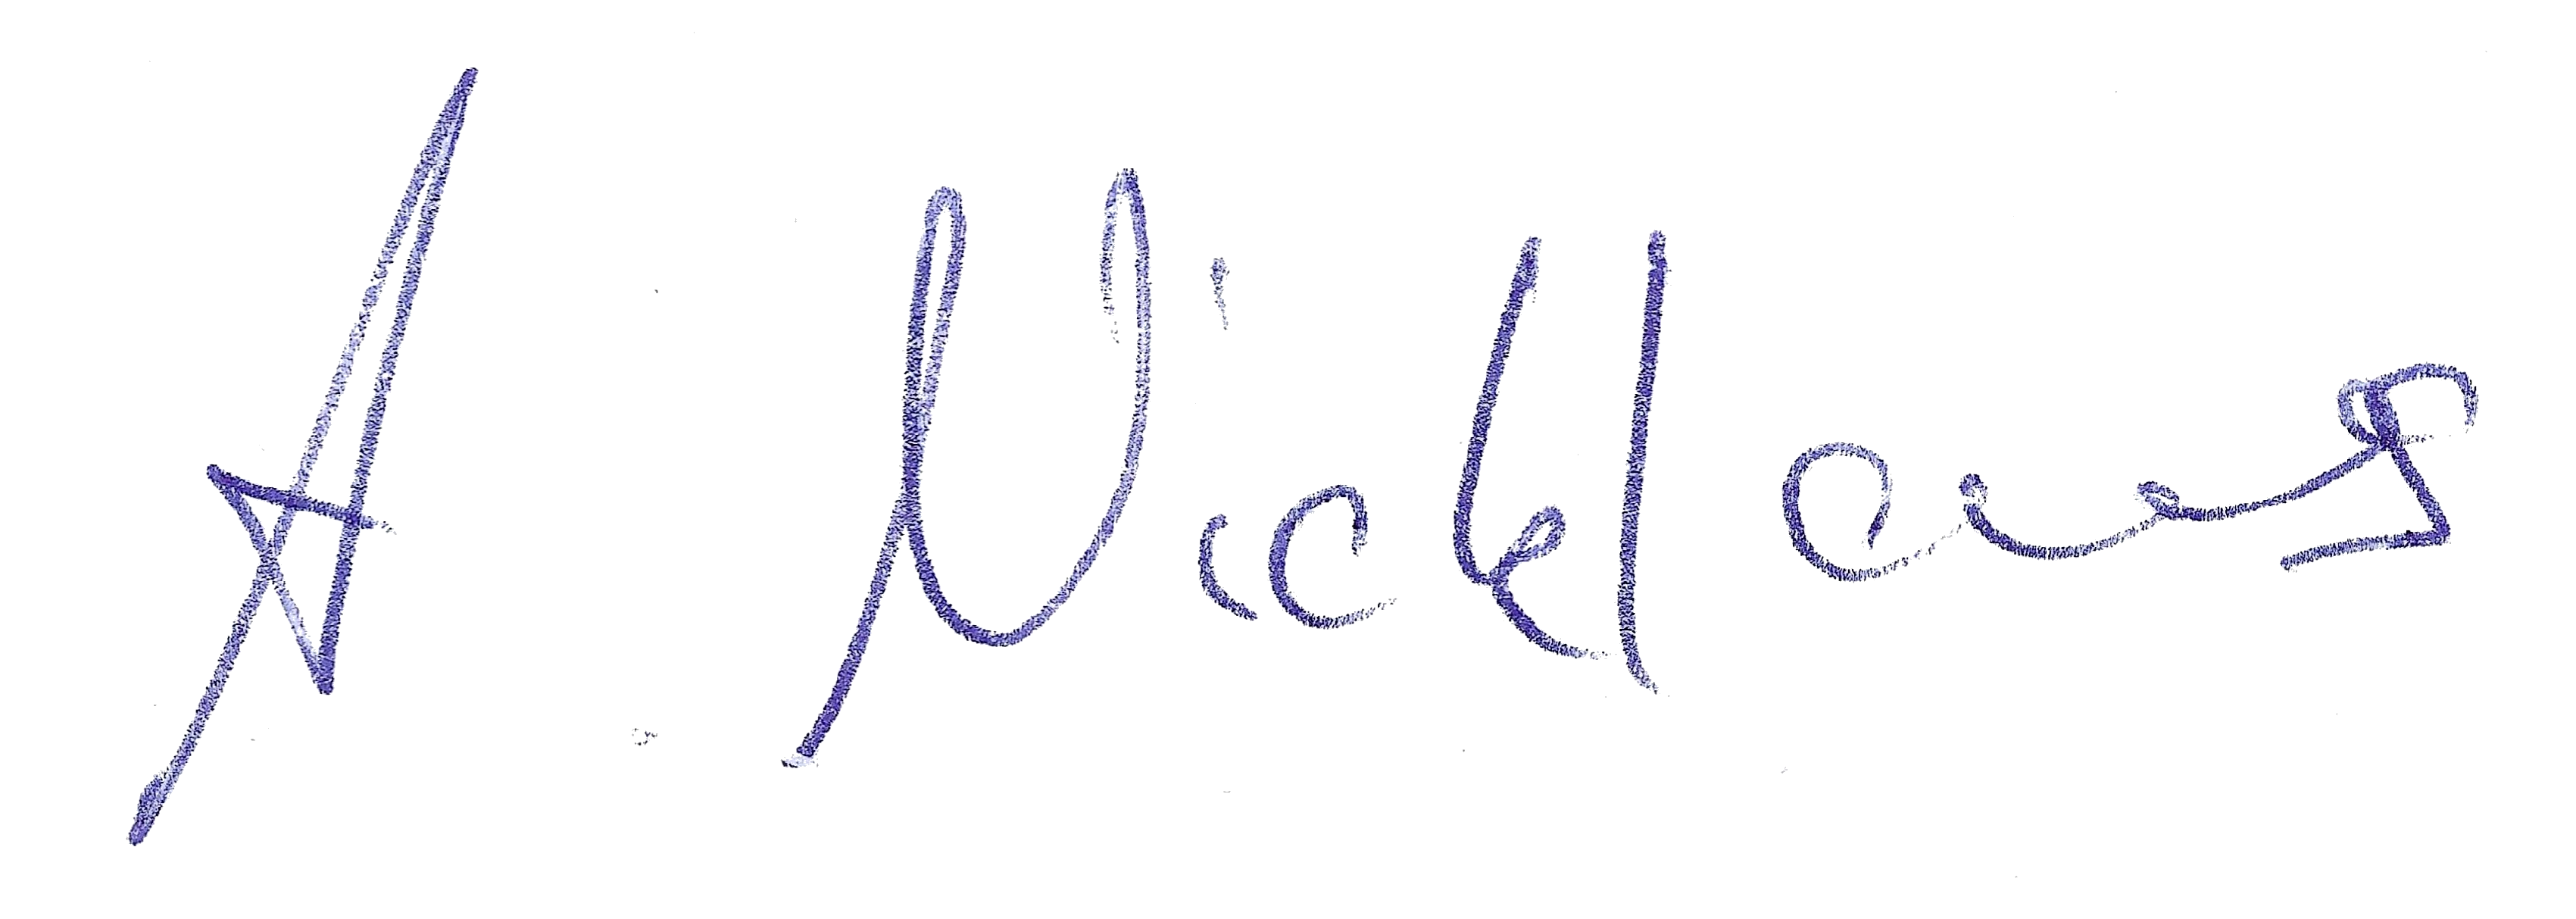
\includegraphics[height=60px]{img/unterschrift.png}
%	\vspace{60px}
	\vspace{10px}
	
	\Author

\pagebreak

\selectlanguage{ngerman}
\begin{abstract}
  Diese Arbeit kurz und knackig.
  % TODO
\end{abstract}

\selectlanguage{english}
\begin{abstract}
  This work in a nutshell.
  % TODO
\end{abstract}

\vfill

\noindent\textbf{Disclaimer:} This paper has been written with the help of AI tools for translating sources and outlining parts of the written content.
All content has been written or created by the author unless marked otherwise.

\pagebreak

\tableofcontents
\pagebreak

\section{Introduction}\label{sec:introduction}
Throughout the evolution of the world wide web, many changes have disrupted the way websites are created.
From simple file servers run by few selected institutions, simple static web pages and dynamic services like blogs and forums to websites created with the help UI tools and web development frameworks, mainly written in JavaScript, development has changed drastically since its beginning.

Older web pages often lacked features, that developers today work with as a matter of course.
Yet their load and rendering most likely would be brazingly fast with today's technological advancements in networking, browser functionalities and user equipment.
Modern websites though are often bigger in size, have a lot more features and are in many respects more complex.
Due to the increased complexity, the mere volume of a webiste's data has increased, especially with more and more multimedia files.
That in return has increased the demand for better performance on all components of the load and rendering process.
This technological advancement has upped the technological sophistication for development tools as well.
Today's modern web development frameworks support developers with tools to create sites and applications through terminal commands.
They often increase the content-per-line-of-code quota through implicit page generation in contrast to the explicit writing of source code from earlier times.
Many frameworks even feature configuration options for directly hosting the webpage.

As the generation process changed from writing code manually to automatically, this implicit page generation undoubtedly increased speed through faster content generation and a greater developer experience for some developers.
Because developer experience varies between different frameworks and some approaches are more intuitive to respective developers, a current trend has evolved for developers to become experts in a single framework rather than many.
This trend leads to a tribal conflict as to which framework is better than others with each tribe being convinced that their framework is the best.
There is no apparant way to determine a \enquote{best framework} in terms of Developer Experience because it is a subjective criterion.
The performance of a framework as assessed by the developer can be similar or greatly different, depending on the frameworks and the interviewees.

When it comes to User Experience and especially the Perceived User Experience however, there are plentiful collections of metrics and criteria to choose from so as to determine the performance of websites, not frameworks.
The optimization of websites has become a goal during development because it has a real effect on both the ranking of web pages in search engines and the user behavior.
Both effects create business interests and financial incentives to invest resources into performance optimization.
However, the lack of research on the topic suggests either a consensus for a negligible effect of the development framework on the website's performance or a lack of knowledge of the effect.
Measurements on the effect of the development framework are a major convoluted task simply because the performance of a specific website can be dependent on many other factors such as the user's device, browser, networking hardware or server-side hardware.
The number of possible combinations of factors and their reliability makes it difficult to measure a single performance run with a reliable result.
Every single result is only a small part of a large number of possible performances the same application could achieve with different parameters.
It is therefore perceivable that a \enquote{perfect combination} of hard- and software exists for each framework or in general, but it is currently not possible to find such a combination because the necessary data is missing.

Many modern web tracking services provide data about the user, the user's devices, current page load times and so on.
This data is helpful in determining current poor performances and therefore possible starting points for optimization efforts.
But it gives very little information about recommended actions or recommended choice of frameworks for a redesign of a web application.
Relying on marketing material for choice of frameworks is equally questionable because most modern frameworks claim to be fast, easy to use and performance efficient.
This suggests that each would be a great choice for developers.

In order to find a suitable framework for an application, a set of metrics needs to be at least outlined for comparison.
Many former studies suggest metrics to be relevant for the User Experience or Search Engine Optimization.
Content metrics such as word count or presence of meta tags might be important for some performance measurements, but might also have no effect on the User Experience.
In contrast, rendering metrics such as page load time or page weight might be ascribed to the framework used during development.

The performance of a framework towards the user can very rarely be compared because there are no publicly available comparisons between exact replicas of web applications built with different frameworks.
Therefore, a comparative study between the same website built with different frameworks is needed to get as close as possible to an exact website replica.
With this data, an informed choice might be made for other projects.

The goals of this paper are to propose a set of metrics that allow comparing mainstream JavaScript frameworks for web applications, to provide a comparative study between selected frameworks and create a tool to compare the rendering performance of a page as a whole and of dynamic components within a page.

\section{Related Work}\label{sec:relatedwork}
\section{Design}\label{sec:design}

Whereas the following chapters cover the implementation of testing and evaluation of results, this section introduces the concept of the comparative study.
The goals of and requirements for the example application, the differences and choices for the hosting environments for testing and the tools for testing as well as selected metrics will are described here.

\subsection{Example Application}\label{subsec:exampleapplication}
% What goals does should the example app fulfil?
% What parts does the example app consist of?
% What requirements does the app cover?
%
% 1. App Idea
% 2. Pages
% 3. Page intention & type
% 4. Multimedia Files & Video Autoplay
% 
% MOSCOW-Analyse
% UML-Diagramme: Services, Pages, Entities

The example application for the study is designed to be a benchmark application for testing.
The following goals were considered during the design process:

\begin{enumerate}
  \item \textbf{Page types}: With the goal of covering most kinds of webpages, three types were identified based on the time of data loading.\label{enum:pagetypes}
  These types differ in timing at which the \acrshort{dom} content is loaded or updated.
  The definition of a finished load or update for this work is that the linking of resources does constitute a finished load or update of the webpage regardless of the load time of said resource.
  The only condition for that is that any linked resource does not update the \acrshort{dom} in any way.
  If a resource does, then the load or update is considered not finished.
  % TODO: WOW! Ändere die obere Definition noch mal
  \begin{enumerate}
    \item Static pages are webpages which do not change their content after the initial response from the web server.
    The initial \acrshort{html} document already is the only resource that is necessary to create a complete \acrshort{dom}.
    If inline skripts update the DOM, they are considered external resources.
    \item Delayed pages do not have a complete \acrshort{dom} after loading and parsing of the initial \acrshort{html} document.
    Some data or content is loaded and inserted (or removed) into the \acrshort{dom} after the initial render.
    The time of these updates can be any time after the initial render, but the execution of code or start of request for the resource that is responsible for the update has to be directly or indirecly triggered by the content of the initial \acrshort{dom} or \acrshort{html} document.
    \item Dynamic pages can be updated or update themselves by events that are not triggered by the content of the initial \acrshort{dom} or \acrshort{html} document.
    These events can either be triggered by user interaction or other events such as websocket messages.
    The time of such updates is by their nature not predictable.
    Dynamic pages are either static or delayed with additional possibilities for updates.
  \end{enumerate}
  This list is created with the knowledge that frameworks or other technology such as caching may move a webpage from one type to another.

  \item \textbf{Modern Development Practices}: The example application should contain modern development practices that do project onto the \acrshort{dom}.
  Practices that have no effect on either the projection of data or user interaction, such as coding styles or project management, are considered to have no effect the performance of the page.
  
  \begin{enumerate}
    \item Components: All pages of the app have to consist of components that encapsulate reproducable \acrshort{html} snippets and may project data onto the \acrshort{dom}.
    \item List iteration: Because iterating long lists may decrease performance noticably, some components or pages should implement list iteration.
    \item String interpolation: Although it is not considered a performance issue before testing, string interpolation is prevalent in all modern frameworks known to the author.
    \item Services: \label{enum:services} Separation of functions in services is wide spread practice to reduce code duplicates and easy refactoring.
    In this case, services also allow to intentionaly implement delays for testing purposes.
  \end{enumerate}
  
  \item \textbf{\acrshort{css}}: Even though the usage of \acrshort{css} can in no way be considered a modern practice, it is still used on effectively every webpage. % TODO: source for effectivvely every webpage
  Additionally, stylesheets are considered render-blocking resources that impact performance negatively. % TODO: source for render-blocking resource
  For this purpose, \acrshort{css} shall be implemented for both pages and components.
  
  \item \textbf{Rendering time}: In addition to page type depending on the time of data load, the machine and time of composing the \acrshort{dom} is dependent on the content availability.
  For this paper, three different types are considered:
  \begin{enumerate}
    \item \acrfull{csr}: The initial request gets a response with a mostly empty \acrshort{html} document (\enquote{skeleton}) except linked \acrshort{css} and \acrshort{js} resources which after loading, parsing and execution update the \acrshort{dom}.
    \item \acrfull{ssr}: Updates that happen after receiving the skeleton through \acrshort{js} code execution on \acrshort{csr}, happen before the initial request is responded to on the web server.
    The initial \acrshort{html} document is filled and no longer a skeleton with \acrshort{ssr}.
    Therefore, it has greater byte size.
    \acrlong{ssr} requires an \enquote{active} front-end server rather than only a file server to execute code.
    \item Prerendering: Rendering happens during build time of the application.
    This increases the build time and the byte size of the initial \acrshort{html} document, but only a file server is needed for hosting.
  \end{enumerate}

  \item \textbf{Multimedia}: Most of network load and therefore network delay is made up by multimedia files. % TODO: source
  Although compression has gotten better over time, the byte size made up by multimedia files of a webpage has gotten larger over the last years. % TODO: source
  Therefore, size optimization of image and video files is considered a major part of performance optimization and a great potential for a performance increase by the used framework.

\end{enumerate}

Based on these considerations, the application \enquote{NotInstagram} was designed as a comparable example application.
It is heavily inspired by Instagram and a partial reproduction of its app design. % TODO: source to IG
\enquote{NotInstagram} consists of four pages (see figure \ref{fig:screenshots}).
\ref{subfig:index} shows the design of the Feed page.
It is the start page of the app and contains 4 parts: the header, the profile list, the post list and a footer.
Each item of the feed page is to be implemented as its own component or components.
The plus icon in the header links to the create page, the footer links to the about page and every instance of a profile picture and profile name links to a profile page.
The later contains profile information including a profile picture, name, user handle / ID, profile creation time, caption and a grid of all the user's posts (see figure \ref{subfig:user}).
The profile component encapsulates all \acrshort{html} elements of that page except the header containing the app logo and X icon, which both link back to the feed page.
Both the feed page and the profile page are generally expected to classify as delayed pages, because the content of profile and posts lists can only be loaded after the page load.

The Create page (see figure \ref{subfig:create}) has three parts.
The header contains the app's logo and a X icon linking to the feed.
A form with three \verb|<input>| elements and a \verb|<button>| element allows the input of an multimedia source (image or video) and a text caption.
The multimedia source can either be an URL or a selection from a list of preuploaded files.
The post caption is a pure text input.
The lower part of the page is the post preview, in which some predefined information such as user profile and the user inputs are combined.
As such, the profile page is a static page until the user uses the creation form, at which point is has to be considered a dynamic page.
The About page (see figure \ref{subfig:about}) is designed to statically display information about the application.
It is a static page because no content is loaded after a delay and no user inputs are possible.

With these pages all \hyperref[enum:pagetypes]{page types} are covered for testing.
The About page and Create page are static, whereas the Feed page and Profile page are partly static (header and footer), but mostly delayed.
The Create page is the only page with dynamic content.

\begin{figure}[ht!]
  \begin{subfigure}{0.49\linewidth}
    \begin{center}
      
\includegraphics[width=\linewidth, height=0.3\textheight, keepaspectratio]{img/ig-clone/Feed.png}
      % TODO: Plus-Icon im Screenshot fehlt
    \end{center}
    \caption{Feed / Index Page (/)}\label{subfig:index}
  \end{subfigure}
  \begin{subfigure}{0.49\linewidth}
    \begin{center}
      
\includegraphics[width=\linewidth, height=0.3\textheight, keepaspectratio]{img/ig-clone/Informationsseite.png}
      % TODO: Profilseite
    \end{center}
    \caption{Profile Page (/user/@PeterPoster)}\label{subfig:user}
  \end{subfigure}
  \begin{subfigure}{0.49\linewidth}
    \begin{center}
      
\includegraphics[width=\linewidth, height=0.3\textheight, keepaspectratio]{img/ig-clone/Beitrag erstellen.png}
      % TODO: X-Icon fehlt
    \end{center}
    \caption{Create Page (/create)}\label{subfig:create}
  \end{subfigure}
  \begin{subfigure}{0.49\linewidth}
    \begin{center}
      
\includegraphics[width=\linewidth, height=0.3\textheight, keepaspectratio]{img/ig-clone/Informationsseite.png}
      % TODO: Backlink fehlt
    \end{center}
    \caption{About Page (/about)}\label{subfig:about}
  \end{subfigure}
  \caption{Screenshots of the NotInstagram application's pages (path in parentheses) \textcolor{red}{(Bilder müssen noch geändert werden)}}\label{fig:screenshots}
\end{figure}

The data fetching and loading is designed to be implemented as \hyperref[enum:services]{services}.
For NotInstagram two different services are needed.
The PostService is a service for all components to query posts.
The method \verb|getAll()| returns a list of all posts by all users and \verb|getByUserHandle(handle)| returns the same list filtered by those posted by a user with the handle equal to the function parameter.
ProfileService is a service to query user profiles.
It has the same two methods which return all user profiles and only one user profile respectively.
Services are designed asynchronous, but the data is not queried from a server external to the browser, but hard coded.
This design decision is based on the premise that delay can be coded into or out of asynchronous functions to mimic network delay for testing purposes if necessary.

Figure \ref{fig:uml} describes the usage of components and services within page views.
It displays the four pages of NotInstagram as views, the two services and 15 components.
Seven of those components are icon components.
Those components serve as wrappers for \acrshort{svg}s to ensure their correct scale and style.
\verb|XIcon| poses an exception to the design as it is a wrapper for a \verb|PlusIcon| component rotated by 45°.
The colored arrows show the usage of one of the services.
Both \verb|FeedView| and \verb|ProfileView| use both services to load data.
For the Feed page, both \verb|PostService.getAll()| and \verb|ProfileServices.getAll()| are needed to pass the data to \verb|PostList| and \verb|ProfileList|.
Notably, each \verb|Post| component accesses the ProfileService again, to get the profile image and name for its headline, even if the information is available in a parent or grandparent component.
Figure \ref{fig:classes} displays the connections between post and profile object instances.
The member \verb|userhandle| of a post references the member \verb|handle| of a user profile.
The Profile page needs access to the service to get the information of the requested profile and a list of posts from the \verb|getByUserHandle| methods to pass into the \verb|Profile| component.
\verb|LogoHeader|, \verb|NotInstagramLogo| and \verb|InfoBlock| are not data-presenting components, but rather styling components.
Their only function is styling text or projecting \acrshort{html} elements with \acrshort{css} information.

\begin{figure}
  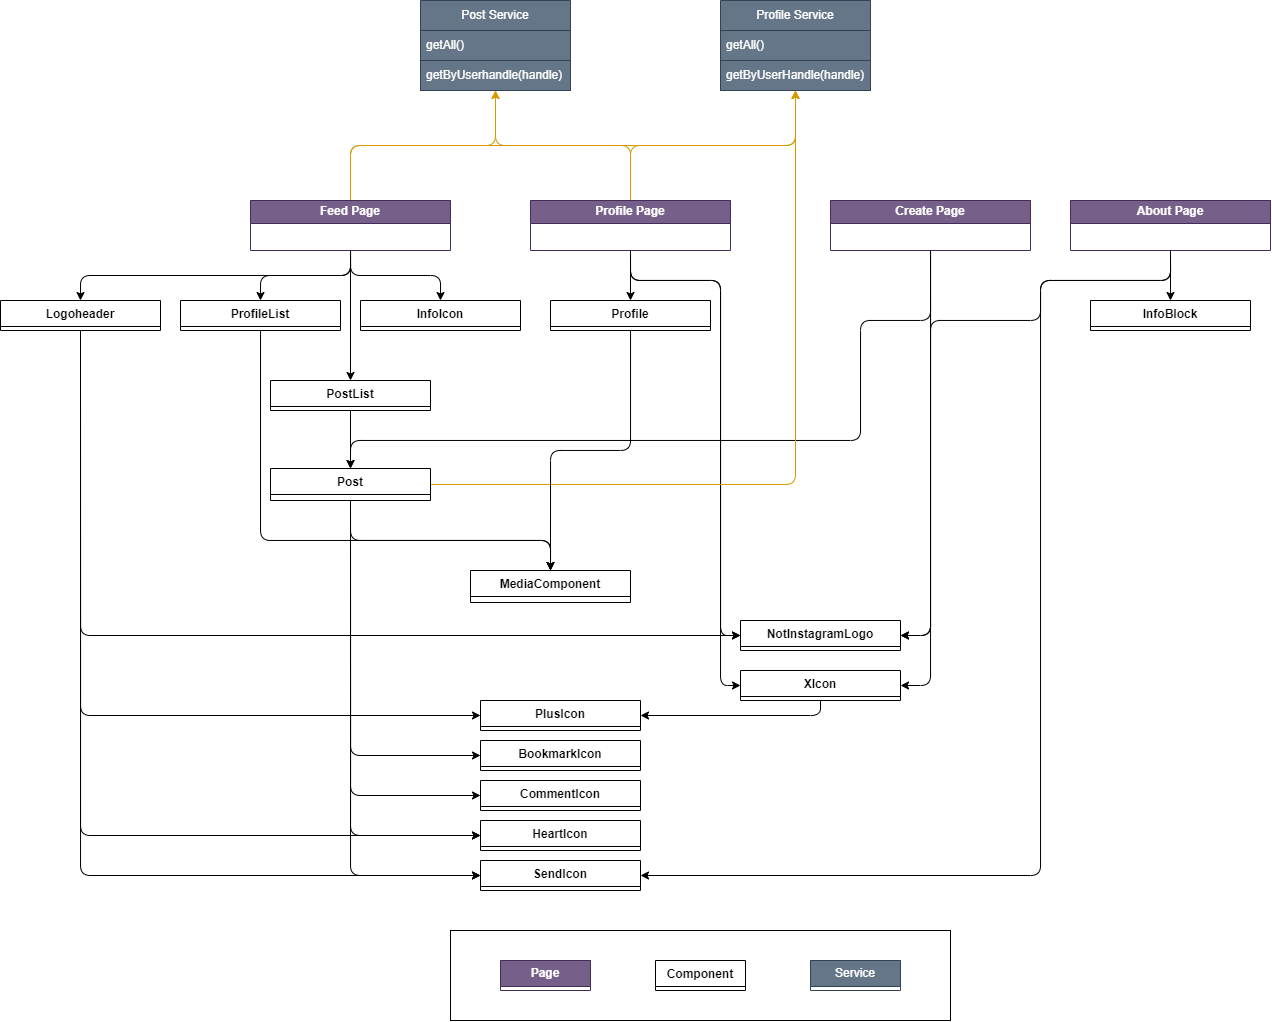
\includegraphics[width=\linewidth]{diagrams/uml.png}
  % TODO: LogoHeader references NotInstagramLogo
  \caption{Pages, Components ands Services of the NotInstagram application}\label{fig:uml}
\end{figure}
\begin{figure}
  \begin{center}
    
\includegraphics[width=0.5\linewidth]{diagrams/entities.png}
  \end{center}
  \caption{Classes used by the NotInstagram services}\label{fig:classes}
\end{figure}

In contrast, the \verb|MediaComponent| is designed as a way to allow both internal and external images and video source.
It is used by \verb|ProfileList|, \verb|Post| and \verb|Profile| to display posts and profile images.
It's main goals is to decide based on the passed image source string how to project the multimedia file onto the \acrshort{dom}.
The component accepts source strings for images and videos, differentiated against by the string's ending and therefore the file's extension.
If it is a local image, namely an image that was available for optimization at build time, the best available form of optimized \verb|<img>| tag should be used.
For external image links starting with \enquote{http://} or \enquote{https://} a less optimized or unoptimized \verb|<img>| tag shall be inserted into the \acrshort{dom}.
For videos, any source string is to be projected onto a \verb|<source>| tag with identical \verb|<video>| wrapper.

The application referres to local images, which can possibly be optimized, and external images, which cannot be optimized.
The reason for this is the assumption for this project that optimizing multimedia files uploaded by a user and referencing them in a manner suitable for this application is not suitable for this work.
Rather, the better alternative for serving the use case of the application would be a dedicated server for encoding, decoding and generally optimizing multimedia files.
Since this solution would be independent from the front-end framework's performance and it would outgrow the scope of this work, a distinction is only made between static images, called local images here, and external images with full URLs.

\subsection{Choice of frameworks}
% Which frameworks were chosen to test?
% Why were these frameworks chosen?
% Which frameworks/tools were considered

The choice of tested frameworks for this study is the choice for which frameworks the application will be implemented in and tested.
The requirements for this selection are twofold.
The application has to be implementable as designed above with the framework without the use of any other non-native tool to the framework or any tool that was not officially intended to be used in combination by the developers of the primary framework.
Additionally, the application must be implementable in JavaScript.
This requirement includes TypeScript frameworks because it is possible to use JavaScript in TypeScript applications. % TODO: source
Ease of use and developer experience should explicitly not influence the selection process because it is part of the evaluation of the frameworks.

Because research revealed in early stages of the study that many frameworks fulfil those requirements, the long list of candidates had to be sorted.
The deciding factor for this selection was usage, awareness of and positive sentiment towards tools among developers because the evaluation of mainstream and general-purpose frameworks appear more valuable than lesser known or specialised tools.
A ranking of the most-used JavaScript front-end frameworks of 2023 \citep{stateOfJs2023} lists the four frameworks with the most developers who have used it before: React (84\%), Vue.js (50\%), Angular (45\%) and Svelte (25\%).
In addition, Astro was chosen for its especially high awareness among the category \enquote{other front-end tools} (30\%), as well as its usage (19\%) and interest (62\%) in the category \enquote{meta-frameworks}.
From the last category of tools, two other frameworks were selected: Next.js and Nuxt.
Both tools are highly-used frameworks and have the appearance and goal of improving React and Vue.js, respectively.
For this reason, they are interesting choices for this study.
All selected frameworks fulfil the requirements.
The application is implementable with all frameworks or intended addition of tools.
Next.js and Nuxt require the usage of React or Vue tools and dynamic components cannot be written in pure Astro. % TODO: source
Astro intends the usage of other frameworks to implement so-called \enquote{islands}.
For those components, React was chosen for its top usage rate.

Other frameworks were also considered for selection.
Solid and Qwik seemed fitting candidates  in this study because of high interest among developers and apparent potential for fast performance of their end product.
Additionally, from the ranking of most-used front-end frameworks Preact was considered with a usage percentage of 13\%.
Ultimately, all three were not chosen because of negative sentiment or low usage among developers.
This concludes the framework selection for this study.
Table \ref{tab:frameworks} list the selection and categorizes them into groups with and without \acrshort{csr} and \acrshort{ssr}.
It also states whether the developer for the application had any previous experience working with the framework.
This information is important for the unintended performance optimizations and can later be used for interpretation of the frameworks performance measurements.
Plus, it will influence the assessment of ease of use and developer experience.

\begin{table}
  \begin{center}
    \begin{tabular}[h]{l c c c }
      \textbf{Framework} & \textbf{\acrshort{csr}} & \textbf{\acrshort{ssr}} & \textbf{Previous Experience} \\ \hline
      Angular & yes & no & yes \\ \hline
      Astro   & yes & yes & yes \\ \hline
      Next.js & no & yes & no \\ \hline
      Nuxt    & yes (generate) & no (build) & no \\ \hline
      React   & yes & no & yes \\ \hline
      Svelte  & yes & no & no \\ \hline
      Vue.js  & yes & no & yes \\ 
    \end{tabular}
  \end{center}
  \caption{List of selected frameworks. Items with both CSR and SSR render some pages or components upon request, but also require CSR}\label{tab:frameworks}
\end{table}


\subsection{Hosting Environments}\label{subsec:hostingenvironments}
% Based on former work, networking plays a vital role in performance and load times
% 
% What exactly should be tested?
% What requirements do the environments have to cover?
% What properties should be considered for the environments?
% TODO: what are the most used hosting environments?
% 
% 1. Vercel
%    1. Reason
%    2. Problems
%    3. Solutions
% 2. Local
%    1. Reason (Network delay)
%    2. Problems

After designing the application, the next step in the study process was to decide on where the application is to be hosted for testing.
Network delay is a great part of render delay and performance issues % TODO: source
because loading files in sequence will block rendering if parsing documents and executing code is dependent on network requests.
The request delay is based on the speed of the web server, the size of the generated file, request and response and the network speed.
Therefore the time needed for fulfilling network requests should be considered in the choice of hosting environment or service.

\begin{figure}
  \begin{center}
    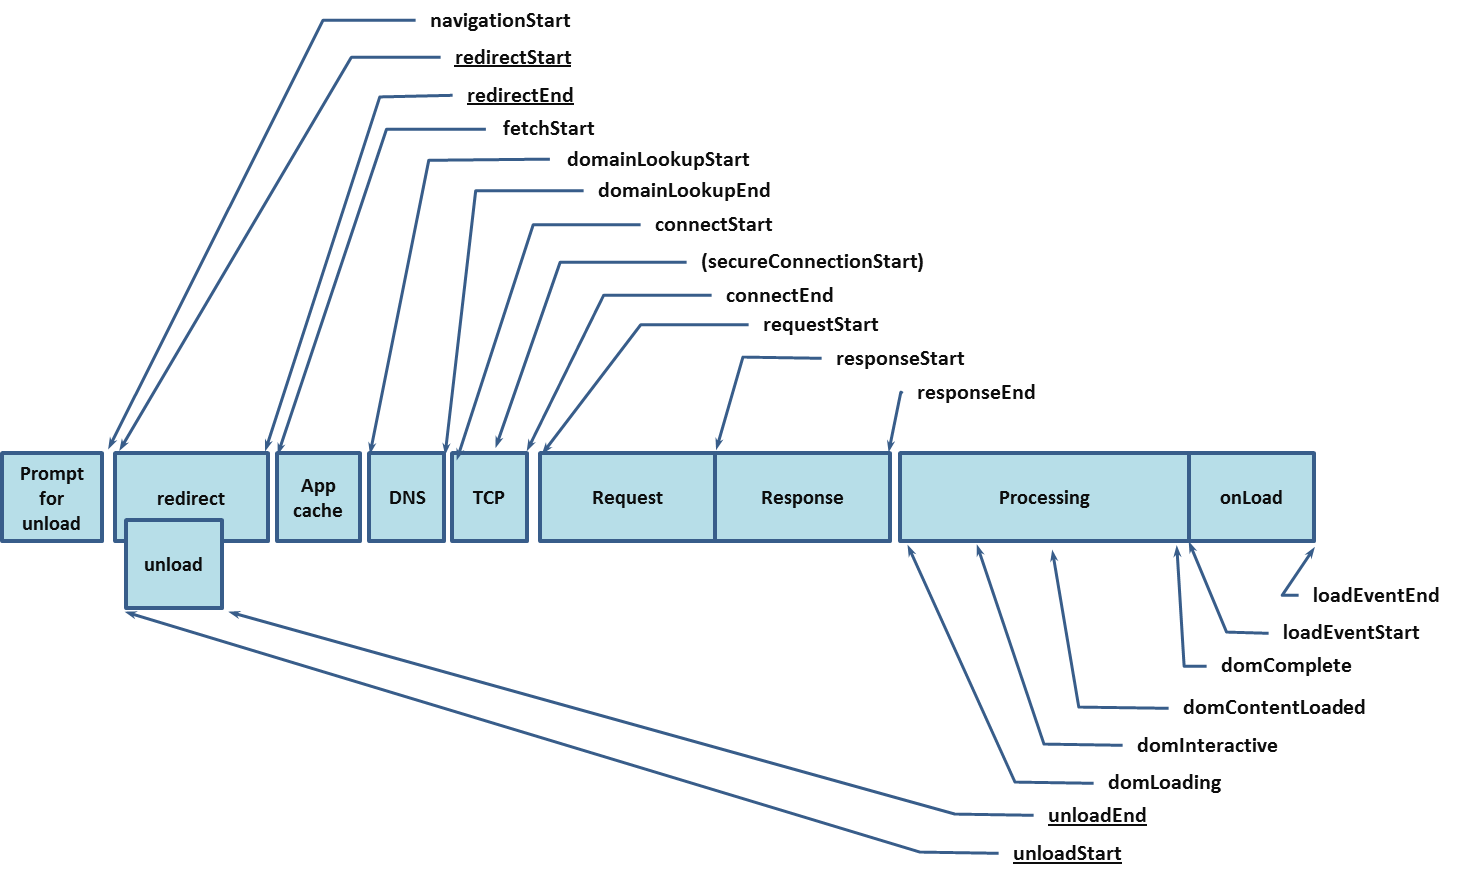
\includegraphics[width=\linewidth]{img/request-timing.png}
  \end{center}
  \caption{Timing attributes defined by PerformanceTiming interface and the PerformanceNavigation interface}\label{fig:timing} %TODO: source https://www.w3.org/TR/navigation-timing/
\end{figure}

Figure \ref{fig:timing} illustrates how a slow network may delay the rendering process of a webpage.
The tests for this study shall cover real-world hosting using publicly available services and local hosting to both test the network delay and test the application without interference of network speeds.
Additionally, tests can not be done only on local servers because tests shall include timings before responseEnd.
Requirements for the distant hosting environment or service are threefold.
The service shall have \enquote{active server capabilities}, meaning capabilities that exceed pure static fileserver functions for \acrlong{ssr} and similar functionalities.
Furthermore, it is required to be a widely used hosting service to ensure the real-world applicability of the study.
Since this requirement is not clearly applicable, it is considered a guideline.
Lastly, to be applicable for small projects as well as established larger websites the service chosen fo the study is required to support free usage and integration into a \acrfull{cicd} configuration because it is a widely used development practice. % TODO: source for "widely used"
As such, the integration is important to require the least possible manual configuration for hosting the application because this study is not supposed to be about the configurability.
Rather, the study shall focus on the "out of the box" performance of the frameworks.
Continuing with that sentiment, the optimization and therefore configuration of the hosting environment is not part of this work.
This is the methodology for answering the question: With which framework do developers get the best performance for their web applications without spending much or any time with optimization and configuration?

Based on these considerations and personal experience with the service, Vercel was chosen for hosting the application for this study.
Vercel supports predefined configurations and automatic recognition of all frameworks chosen for this study.
Also, Vercel projects integrate seamlessly into a \acrshort{cicd} process based on its integration with Github.
A Github repository was created for each framework and connected to a Vercel project.
During initialization of the Vercel projects and first preliminary tests, one problem with Vercel's free account quickly became apparent:
The bandwidth limitation of 100GB per month and account was reached after two weeks of testing unoptimized and unfinished versions of the applications with large image and video files.
Because no information was found on the effect of a reached limit, the account was deemed dead for the month.
The solution to this problem was the creation a second free Vercel account and the plan to create another account every time the limit would be reached in the future, which it did not.

The second hosting environment for this study is hosting the application locally on the testing machine.
This environment ensures minimal network load times and eliminates every other connected delays such as resolving domain names.
If the framework supports a \enquote{preview} mode, it was used for hosting the application.
Otherwise, the application would be build and hosted using the \verb|serve| command or the active server would be started with \verb|node <filename>|.
If neither of the two options would be available, the \enquote{dev} mode of the application would be used and tested.
Table \ref{tab:hostCommands} lists the used commands for building and starting the webserver per framework.

\begin{table}
\begin{center}
  \begin{tabular}[h]{| l | l | l |}
    \hline
    \textbf{Framework} & \textbf{Build Command} & \textbf{Host Command} \\ \hline
    Angular & \verb|ng build| & \verb|serve| \\ \hline
    Astro & \verb|astro build| & \verb|astro preview| \\ \hline
    Next & \verb|next build| & \verb|next start| \\ \hline
    Nuxt & \verb|nuxt build| & \verb|nuxt preview| \\
     & \verb|nuxt generate| & \verb|nuxt preview| \\ \hline
    React & \verb|react-scripts build| & \verb|serve| \\ \hline
    Svelte & \verb|vite build| & \verb|vite preview| \\ \hline
    Vue & \verb|vite build| & \verb|serve| \\ \hline
  \end{tabular}
\end{center}
\caption{Build and host command for each used framework as used for testing the applications hosted locally}\label{tab:hostCommands}
\end{table}

\subsection{Performance Metrics}
% What metrics can be measured?
% What metrics should be used?
% What metrics will be used?
% 
% 1. Lighthouse performance
% 2. Page weight
% 3. Largest/First Contentful/Meaningful Paint
% 4. TTFB/TTI/SpeedIndex

The load time and reactivity of a web page and its user interface decreases user retention and continuing user actions over time independently from the content. %TODO: source
The \enquote{reaction time} is interpreted in three separate ways for this study: The page load time, meaning the time from navigation start to \acrshort{dom} mutation, the time from a state change, e.g. data query end, to \acrshort{dom} mutation, here called component load time, and the time between a user input to finished \acrshort{dom} mutation, called component update time for this study.
Nearly most of these times can be combined from or described using navigation events (see figure \ref{fig:timing}).
These timing categories are not exclusive, but measurements for these time categories do overlap.

Naturally, other metrics than the navigation timings were also considered.
From the list of measurements in Lighthouse reports (see chapter \ref{subsec:testingtools}), sublists with relevant metrics were created to properly represent the time measurements of the described render sections and DOM mutation events.
These reports cover the initial load of a page and visual content presentation after initial load.
None of the Lighthouse metrics cover the time of \acrshort{dom} mutations after user input events.
Therefore, yet additional measurements have to be considered to describe the performance of mutations.
To this end, some self-written code is injected through Playwright (see chapter \ref{subsec:testingtools}) to measure the time of updates to the \acrshort{dom}.
The following sections describe which measurements are needed for each render section in detail.

\subsubsection{Page Load Times}

In the context of this study, the first contact point for a user to a web page is considered to be the first page load or initial page load.
Within the initial load, the user's main expectations and goals are assumed to be finding a page with the wanted information or input rather than finding the information itself.
As a result, the aim of the client's browser and render engine for this first time frame, called \enquote{page load} here, is to both parse \acrshort{html} and project the content of the page onto the \acrshort{dom}.
In order to focus on this time frame, these metrics describe the application's performance.

\begin{itemize}
  \item \textbf{\acrfull{tbw}}: The total size of files or content of response directly increases either the App Cache time between \verb|fetchStart| and \verb|domLoading| or \verb|domContentLoaded| if the resource can be cached in the client or the response time between \verb|responseStart| and \verb|responseEnd| otherwise.
  \item \textbf{\acrfull{ttfb}}: The time between \verb|navigationStart| and \verb|responseStart|.
  Most of the network delay can be described by the \acrshort{ttfb}.
  Often inaccurately paraphrazed as \enquote{ping}.
  \item \textbf{\acrfull{tti}}: The time until the page can be interactive, described by the \acrshort{dom}'s loading state \enquote{interactive}.
  By navigation events described as the time between \verb|navigationStart| and \verb|domInteractive|.
  Notably, the timing of \verb|domInteractive| is not reliable because a \acrshort{dom} may become interactive, but the browser may not be interactive yet.
  Additionally, resources may still be loading.
  For example, a \acrshort{dom} from a \acrshort{html} skeleton may be \enquote{interactive} after a few milliseconds, but no content may be rendered for the user to see, %TODO: source https://html.spec.whatwg.org/multipage/dom.html#current-document-readiness
  because \acrshort{csr} code is still loading \citep{htmlLivingStandard}.
  \item \textbf{DomContentLoaded}: Similar to \acrshort{tti}, DomContentLoaded measures the time between \verb|navigationStart| and \verb|domContentLoaded|.
  At this point in time, \enquote{all subresources apart from async script elements have loaded} \citep{htmlLivingStandard}.
  A large difference between \acrshort{ttfb} and DomContentLoaded indicates a great size or at least long load time of subresources.
  \item \textbf{LoadEventEnd}: Total time spent imidiately after initial load of a page until the \acrshort{dom}'s onload event is finished.
  This is the time from \\
  \verb|navigationStart| to \verb|loadEventEnd|.
  The time represents both the capability of the used framework to optimize the usage of a client's and network's resources on initial load and the priorization of JavaScript execution by splitting not immediately needed code into async scripts.
  \item \textbf{\acrfull{tbt}}: The total time spent by a browser with parsing and optionally resources that block the rendering process from finishing.
  This includes stylesheets and scripts without the \verb|async| or \verb|defer| tag.
  The metric directly represent the time before the browser can fulfil the user's goal on initial load.
  \item \textbf{\acrfull{lvc}}: Time from \verb|navigationStart| until the last visual change above the fold, meaning within the viewport of the user. %TODO: describe Observed lvc
  \item \textbf{\acrfull{lcp}}: The time between navigation to the page and the time of rendering for the visually largest text or image element in the user's viewport \citep{lcpDocumentation}.
  Optimization of this metric requires and understanding of the page's content and element size within the viewport.
\end{itemize}

From this list of relevant metrics, some expectations can be formulated before testing for them.
First, \acrshort{tbt} is most likely slower with \acrshort{csr} frameworks because the code execution filling the \acrshort{html} skeleton takes some time that is not necessary in client with SSR and Prerendered pages.
On delayed pages this difference is expected to be very slight or nonexistent.
Second, the \acrshort{lcp} probably will not differ across frameworks, but naturally across pages.
In contrast, if a framework does create a faster result for its \acrshort{lcp}, it is expected to be a \acrshort{ssr} or Prerendering framework because of its expected shorter \acrshort{tbt}.
Third, \acrshort{csr} frameworks differ from \acrshort{ssr} and Prerendering frameworks by \acrlong{tbw} similar to \acrlong{lcp}.
Although the \acrshort{html} document is much slimmer with \acrshort{csr}, the \acrshort{js} files are expected to be equally larger than server-side rendered and prerendered pages.
It is probably nearly equal in sum because the byte size of the page is likely mostly made up from multimedia files such as images and videos, \acrshort{css} and \acrlong{js} files. 
Fourth, the selected frameworks should be inversely seperable into groups by the \acrlong{ttfb}.
Most likely \acrshort{csr} and Prerendering frameworks will be faster for this metric because the web server can serve as a static fileserver and does not have to execute any additional code.
Fifth, because \acrshort{csr} pages consist of only nearly empty \acrshort{html} skeletons and links to \acrshort{js} and \acrshort{css} files, the \acrshort{tti} is expected to be much faster for \acrshort{csr} pages.
Lastly, the timing of the \verb|loadEventEnd| is not clearly predictable before testing.
The only expectation is that newer framework perform better in this metric simply because they are newer and are expected to make optimizations that go into a faster parsing and rendering of a web page.

With these expectations it would be most interesting to see the differences between CSR and SSR frameworks.
From the list of selected frameworks for this study, those frameworks with direct competitors are Nuxt compared with Vue.js as well as Next.js in comparison to React.
Additionally, Angular and Svelte in the group of CSR frameworks shall be compared with the SSR framework group with Astro.

\subsubsection{Component Load Times}
% Measuring JS-dependent parts of the webpage
% 
% 1. Dom Updates with MutationObserver
% 2. Problems with MutationObservers and Playwright

As a second category of relevant metrics, measurements for the separation of the app into components are grouped together.
This category is designed to reflect the performance of the \acrlong{js} that was generated by the framework.
This stands in contrast to how much content can be rendered by the time of \verb|responseEnd|.
To this end, only measurements after \verb|responseEnd| can be taken into consideration.
Each mutation from the initial \acrshort{dom} has to be interpreted as a update to a component.
The following metrics are part of this category.

\begin{itemize}
  \item \textbf{LoadEventEnd}: The time between \verb|responseEnd| and \verb|loadEventEnd|.
  It combines all render-blocking parsing and synchronized code execution.
  Therefore, it is a combined indicator from the code performance and general optimization.
  \item \textbf{\acrfull{ofvc}}: The time of the first visual update from a blank canvas.
  It is an indicator for the start of visual rendering and a signal to a user that the page is working or loading.
  For pages with itneractive elements, this metric is less important that the \acrshort{tti}.
  \item \textbf{\acrfull{olvc}}: The time of the last visual update to a web page.
  The metric is the most promisiing for this study as it indicates the end of the perceptable rendering process and therefore perceived load speed.
  \item \textbf{Mutation Times}: Time from initialization of the app with a predetermined \acrshort{html} element such as \verb|<main>| to a \acrshort{dom} mutation.
  See section \ref{subsub:componentUpdateTimes} for more info on this.
  \item \textbf{\acrshort{tbt}}
  \item \textbf{\acrshort{tti}}
\end{itemize}

Based on the intention for testing these metrics, comparing or optimizing \acrlong{js} frameworks, the following expectations were presented before tests.
First, prerendered and \acrshort{ssr} pages are expected to show a earlier \acrshort{fvc} because the execution of any code for delay components can start earlier.
This expectation comes from the added code of \acrshort{csr} applications to add static elements to the \acrshort{dom} through \acrshort{js}.
Second, \acrshort{csr} applications probably finish their \acrshort{lvc} slightly earlier than other applications.
The assumption for this prediction is that every application starts long tasks only after the \acrshort{html} was parsed which takes longer for \acrshort{ssr} or prerendered pages.
As a result of these two expectations the observations of a \verb|MutationObserver| most likely have a lower maximum and are less spread out for \acrshort{ssr} and prerendered pages, but start later than \acrshort{csr} pages.
Third, as described above, the \acrshort{tbt} is expected to be slightly later for \acrshort{csr} than for \acrshort{ssr} or prerendered applications and fourth, \acrshort{csr} apps should have a slower \acrshort{tti}.

With these metrics, identifying bloated applications and components is the goal.
\acrlong{js} that is loaded, parsed and executed that increases the initial load time of a page should be indicated through these tests.
Such unnecessary or render-blocking scripts are pointed out through \acrshort{tbt} and littele difference between \acrshort{fvc} and \acrshort{lvc}.
For example, a script can be considered unnecessary for initial load if it is executed before rendering that only defines functions, initializes objects that are not yet needed or creates a blocking dependency chain, e.g. through importing another script.

\subsubsection{Component Update Times}\label{subsub:componentUpdateTimes}
% 3rd type of update through JS
% 
% - Interesting comparisons with reasoning and expectation
%   - MPA vs SPA
%   - Angular vs React vs Vue
%   - Nuxt vs Vue und Next vs React
%   - Vue-basiert vs React-basiert
%   - Svelte vs Astro

For the third category of relevant metrics, \acrshort{dom} mutation stemming from events triggered by the user are grouped together.
These event influence the user experience on the condition that they lead to \acrshort{dom} mutations.
Only two kinds of measurements can be made to gain insight into update speed although three measurements are perceivable.

\begin{itemize}
  \item \textbf{User Input Times}: The time of a user input.
  The kind of user input is not restricted to \verb|onInput| or \verb|onChange| events, but rather any event triggered by the user.
  \item \textbf{State Change Times}:The time a state changes after user input.
  This is usually not automatically directly testable because the internal functionality of the framework is not always observable.
  \item \textbf{Mutation Times}:Time of a mutation from user input within a predetermined \acrshort{html} element such as \verb|<main>| to another \acrshort{dom} mutation.
  A \verb|MutationObserver| is initialized and all mutations are recorded. Designated mutations to the \acrshort{dom} are added child elements, removed child elements and attribute updates (added, edited and removed).
\end{itemize}

For these metrics no expectations could be formulated before testing because the speed of an mutation is purely based on the implementation of the framework itself.
These implementations are not openly accessible without knowledge of the frameworks' source code.
Still, some prediction can be made independently from a specific framework.
Apps that represent their state in the DOM, e.g. an \enquote{edited} state for a user input or an updated value attribute of an \verb|<input>| element, will most likely have\dots

\begin{enumerate}
  \item more entries in the recorded \acrshort{dom} mutations and\dots
  \item a later last entry in the recorded \acrshort{dom} mutations.
\end{enumerate}

Also, the implementation of the app shows differences here as additional elements, such as \verb|<div>| elemets as wrappers for each component can influence the time and number of updated elements in either direction, dependent on the use case.
To summarize some comparisons between frameworks or groups of frameworks, the most appealing for the evaluation are the following.

\begin{enumerate}
  \item \textbf{\acrshort{csr} - \acrshort{ssr}}: Before testing, deifferences between \acrshort{csr} and prerendered pages are expected, but the metrics and amount of differences are a probable subject of interest.
  Because there is no perceivable differences between prerendered  pages and server-side rendered pages from a client perspective, they are grouped together in this context.
  \item \textbf{Angular - React - Vue}: Because these \acrshort{csr} frameworks have been competing for \textcolor{red}{X} %TODO: how many years
  years at this point and they are still the most famous front-end frameworks, % TODO: source
  the comparison of these frameworks is relevant for this study.
  \item \textbf{Nuxt - Vue.js}:As a next generation of the Vue.js framework, the actual performance increase of Nuxt is interesting for developers.
  \item \textbf{Next.js - React}: Same as above
  \item \textbf{Vue-based - React-based}: Because a direct comparison of frameworks based on React and based on Vue.js is possible with multiple candidates, a difference in performance is an actual relevant factor for the choice between the ecosystems.
  \item \textbf{Svelte - Astro}: As the most modernly popular frameworks in the selection of frameworks, Astro and Svelte have the potential to both outdo their contenders and outdo each other.
  This comparison is most interesting for fans of new tools and the development teams of the frameworks themselves.
\end{enumerate}

\subsection{Testing Tools}\label{subsec:testingtools}
% What tools were using testing and how do they work? 
% What requirements should be fulfilled by the tools
% 
% 1. Introduction into Playwright
% 2. Introduction into Lighthouse CLI
% 
% What problems are expected to arise from these tools?
% What requirements are covered by which tool?

In order to test for these metrics, a set of multiple testing tools is needed.
These testing tools are required to cover the measurements describe above and the tools have to work with similar configuration for all selected frameworks.
Test reports have to be generated in a machine-readable format in order to evaluate the results and create aggregate metrics from them.
This is a requirement because from previous experience it is known that performance values in the web development context have a considerable variance.
To this end, two different tools for automating tests were chosen:

\begin{enumerate}
  \item \textbf{Lighthouse \acrshort{cli}}: The Lighthouse \acrshort{cli} makes it possible to automate the generation of Lighthouse reports.
  Tests for these reports combine measurements with weights in categories and reduce them to a single score, as well as five main category scores.
  These categories are performance, accessibility, best practices, \acrshort{seo} and \acrshort{pwa}.
  Additionally, Lighthouse reports contain recommendations for optimizing metrics and increasing the scores.
  It is a popular tool for measuring the initial page loads, page content and meta information for a web site.
  Changes after the initial page load are not possible to test with the Lighthouse \acrshort{cli}.
  Reports are by default generated as \acrshort{html} files, but the tool was configured to generate both \acrshort{html} and \acrshort{json} reports for this study.
  Since Lighthouse is designed to test live websites in production, the tool does not support starting a local development server.
  Testing with Lighthouse therefore needs to include building and hosting the application locally while tests are running.
  \item \textbf{Playwright}: Playwright is a front-end testing tools for web applications in development.
  It mainly supports checking page content, but also supports the execution of injected \acrlong{js} and full control over the browser.
  This also means that the control over the user inputs enables measurement of timings connected to user behaviour such as clicking links and buttons, hover the mouse over elements or using \verb|<input>| elements.
  Such options are needed to evaluate the timings of interactive elements.
  The development-focused design also bears the advantage of its initialization being included in some framework's initialization options.
  Both Svelte and Vue.js support installing and initializing configuration for Playwright in their own initialization (see chapter \ref{sec:implementation} for more on this).
  Similar to Lighthouse, reports can be created as \acrshort{html} and \acrshort{json} files.
  For this study, only \acrshort{json} reports were used for the results, but \acrshort{html} reports were used for debugging tests.
\end{enumerate}

Although all requirements can be fulfilled with these tools, multiple problems were found with them.
Because Lighthouse reports include data that is influenced by all actors and constraints regarding the web page, many factors contribute to the variability of its results.
\cite{lighthouseVariability} contains a list of sources of variability.
The relevant sublist of factors for this study contains for local tests client resource contention, client hardware variability and browser nondeterminism.
Client hardware variability is mitigated throught the usage of the same client device for all tests.
The client device in question is a HP Envy x360 Convertible 15-eu0xxx with an AMD Ryzen 5 5500U processor and 16GB RAM.
The operating system on the device is Windows 11 Home (Version 10.0.22631) during testing.
Client resource contention could not be fully mitigated.
Attempts to keep a lid on client resources was killing the most hardware intensive background tasks and services on the test machine before starting tests.
Browser nondeterminism was taken into account and adopted as a test dimension because the target group of an application should be factor for the choice of framework, especially for purely desktop or mobile applications.
To this end, tests were executed with the most commonly used browsers wherever possible.
For Lighthouse tests, such an option was not found.
Instead, all tests were explicitly executed on Google Chrome for desktop.
A Lighthouse report was not generated on other browsers.

For tests on a distant server, other factors contribute to the fluctuation of Lighthouse test results in addition.
Local network variability, tier-1 network variability and web server variability have to be considered for the tests.
The first two could not be mitigated.
The internet connection speed at the test location was 100 Mbit/s to simulate common modern consumer internet connections. % TODO: source
Web server variability could not be mitigated as well.
For this reason, a hosting service was explicitly chosen for all tests to minimize the variability across frameworks (see section \ref{subsec:hostingenvironments}).

For mitigation of all factors of variability, Lighthouse tests were executed 20 times to gain an average of all measurements.
The repetitions were configured with the same browser context and web server for local tests for each run.
The reason for this decision is that fluctuations based on the first requests within the client or the server should be mitigated with this method.

Two additional problems with Playwright were found before the start of the test phase.
The time of injection for \acrshort{js} script could not be properly determined.
This fluctuation could not be mitigated.
Also, reading data from the window context after the fact proved to be difficult because the context closes after the test ends and the report only contains explicitly tested values.
Objects such as the needed navigation timings are no longer available after the fact.
The solution to this problem was to attach all necessary information as a file to the report so it is readable after the context closed.

With all tools and workarounds in place, the data needed for the study could be collected.
Lighthouse covers \acrshort{tbw}, \acrshort{ttfb}, \acrshort{tti}, \acrshort{tbt}, \acrshort{lcp}, \acrshort{fvc}, \acrshort{ofvc} and \acrshort{olvc} whereas Playwright cover all naviation and \acrshort{html} event times, namely DomContentLoaded, LoadEventEnd, user input times, state change times and mutation times.


\section{Implementation}\label{sec:implementation} 
% Project creation strategy
% Project separation strategy

\subsection{Components}\label{subsec:components}
% Notable components and HTML elements
% How are they constructed?
% How are they projected onto the DOM?
% 
% 1. MediaComponent
% 2. About Aufbau
% 3. Post mit und ohne Daten
% 4. Astro CreateForm
\subsection{Tests}\label{subsec:tests}
% How are tests configured and implemented?
% What is measured, stored and evaluated?
% 
% - Test categories
%   - Page Load
%   - Dynamic Component Load Times
%   - State Change Times
% - Playwright test configuration
%   - Tests
%   - Attachments
%   - Screenshots
% - Browser Choices: Reasoning and test implementation

\section{Evaluation}\label{sec:evaluation}
\subsection{Page Load Times}\label{subsec:pageloadtimes}
% 1. Which pages load fast?
% 2. How much does much post-rendering-data add to load time?
% 3. Which frameworks creates fast-loading pages?
% 4. Does it match my expectations?

\subsection{Component Load Times}\label{subsec:componentloadtimes}
% 1. Which components load with delay?
% 2. Which frameworks have fast-loading delayed components?
% 3. Do pre-rendered pages even have delayed components?

\subsection{Component Update Times}\label{subsec:componentupdatetimes}
% 1. Which differences can be made out towards [Component update times](#component-update-times)?
% 2. Which HTML-Elements even update?
% 3. Which frameworks update HTML-Elements faster than others?

\section{Conclusion}\label{sec:conclusion}
% 1. Which framework works best with page load times?
% 2. Which framework works best with component load times?
% 3. Which framework works best with component update times?

\section{Summary}\label{sec:summary}

\pagebreak

\appendix
\listoffigures

\listoftables
\glsaddall
\printnoidxglossary[type=\acronymtype,nonumberlist,style=long]

\nocite{*}
\bibliography{sources}{}
\end{document}